\documentclass{ximera}
%% You can put user macros here
%% However, you cannot make new environments

\listfiles

\graphicspath{{./}{firstExample/}{secondExample/}}

\usepackage{tikz}
\usepackage{tkz-euclide}
\usepackage{tikz-3dplot}
\usepackage{tikz-cd}
\usetikzlibrary{shapes.geometric}
\usetikzlibrary{arrows}
%\usetkzobj{all}
\pgfplotsset{compat=1.13} % prevents compile error.

%\renewcommand{\vec}[1]{\mathbf{#1}}
\renewcommand{\vec}{\mathbf}
\newcommand{\RR}{\mathbb{R}}
\newcommand{\dfn}{\textit}
\newcommand{\dotp}{\cdot}
\newcommand{\id}{\text{id}}
\newcommand\norm[1]{\left\lVert#1\right\rVert}
 
\newtheorem{general}{Generalization}
\newtheorem{initprob}{Exploration Problem}

\tikzstyle geometryDiagrams=[ultra thick,color=blue!50!black]

%\DefineVerbatimEnvironment{octave}{Verbatim}{numbers=left,frame=lines,label=Octave,labelposition=topline}



\usepackage{mathtools}


\title{About this Project} \license{CC BY-NC-SA 4.0}



\begin{document}
\begin{abstract}
\end{abstract}
\maketitle

\begin{image}
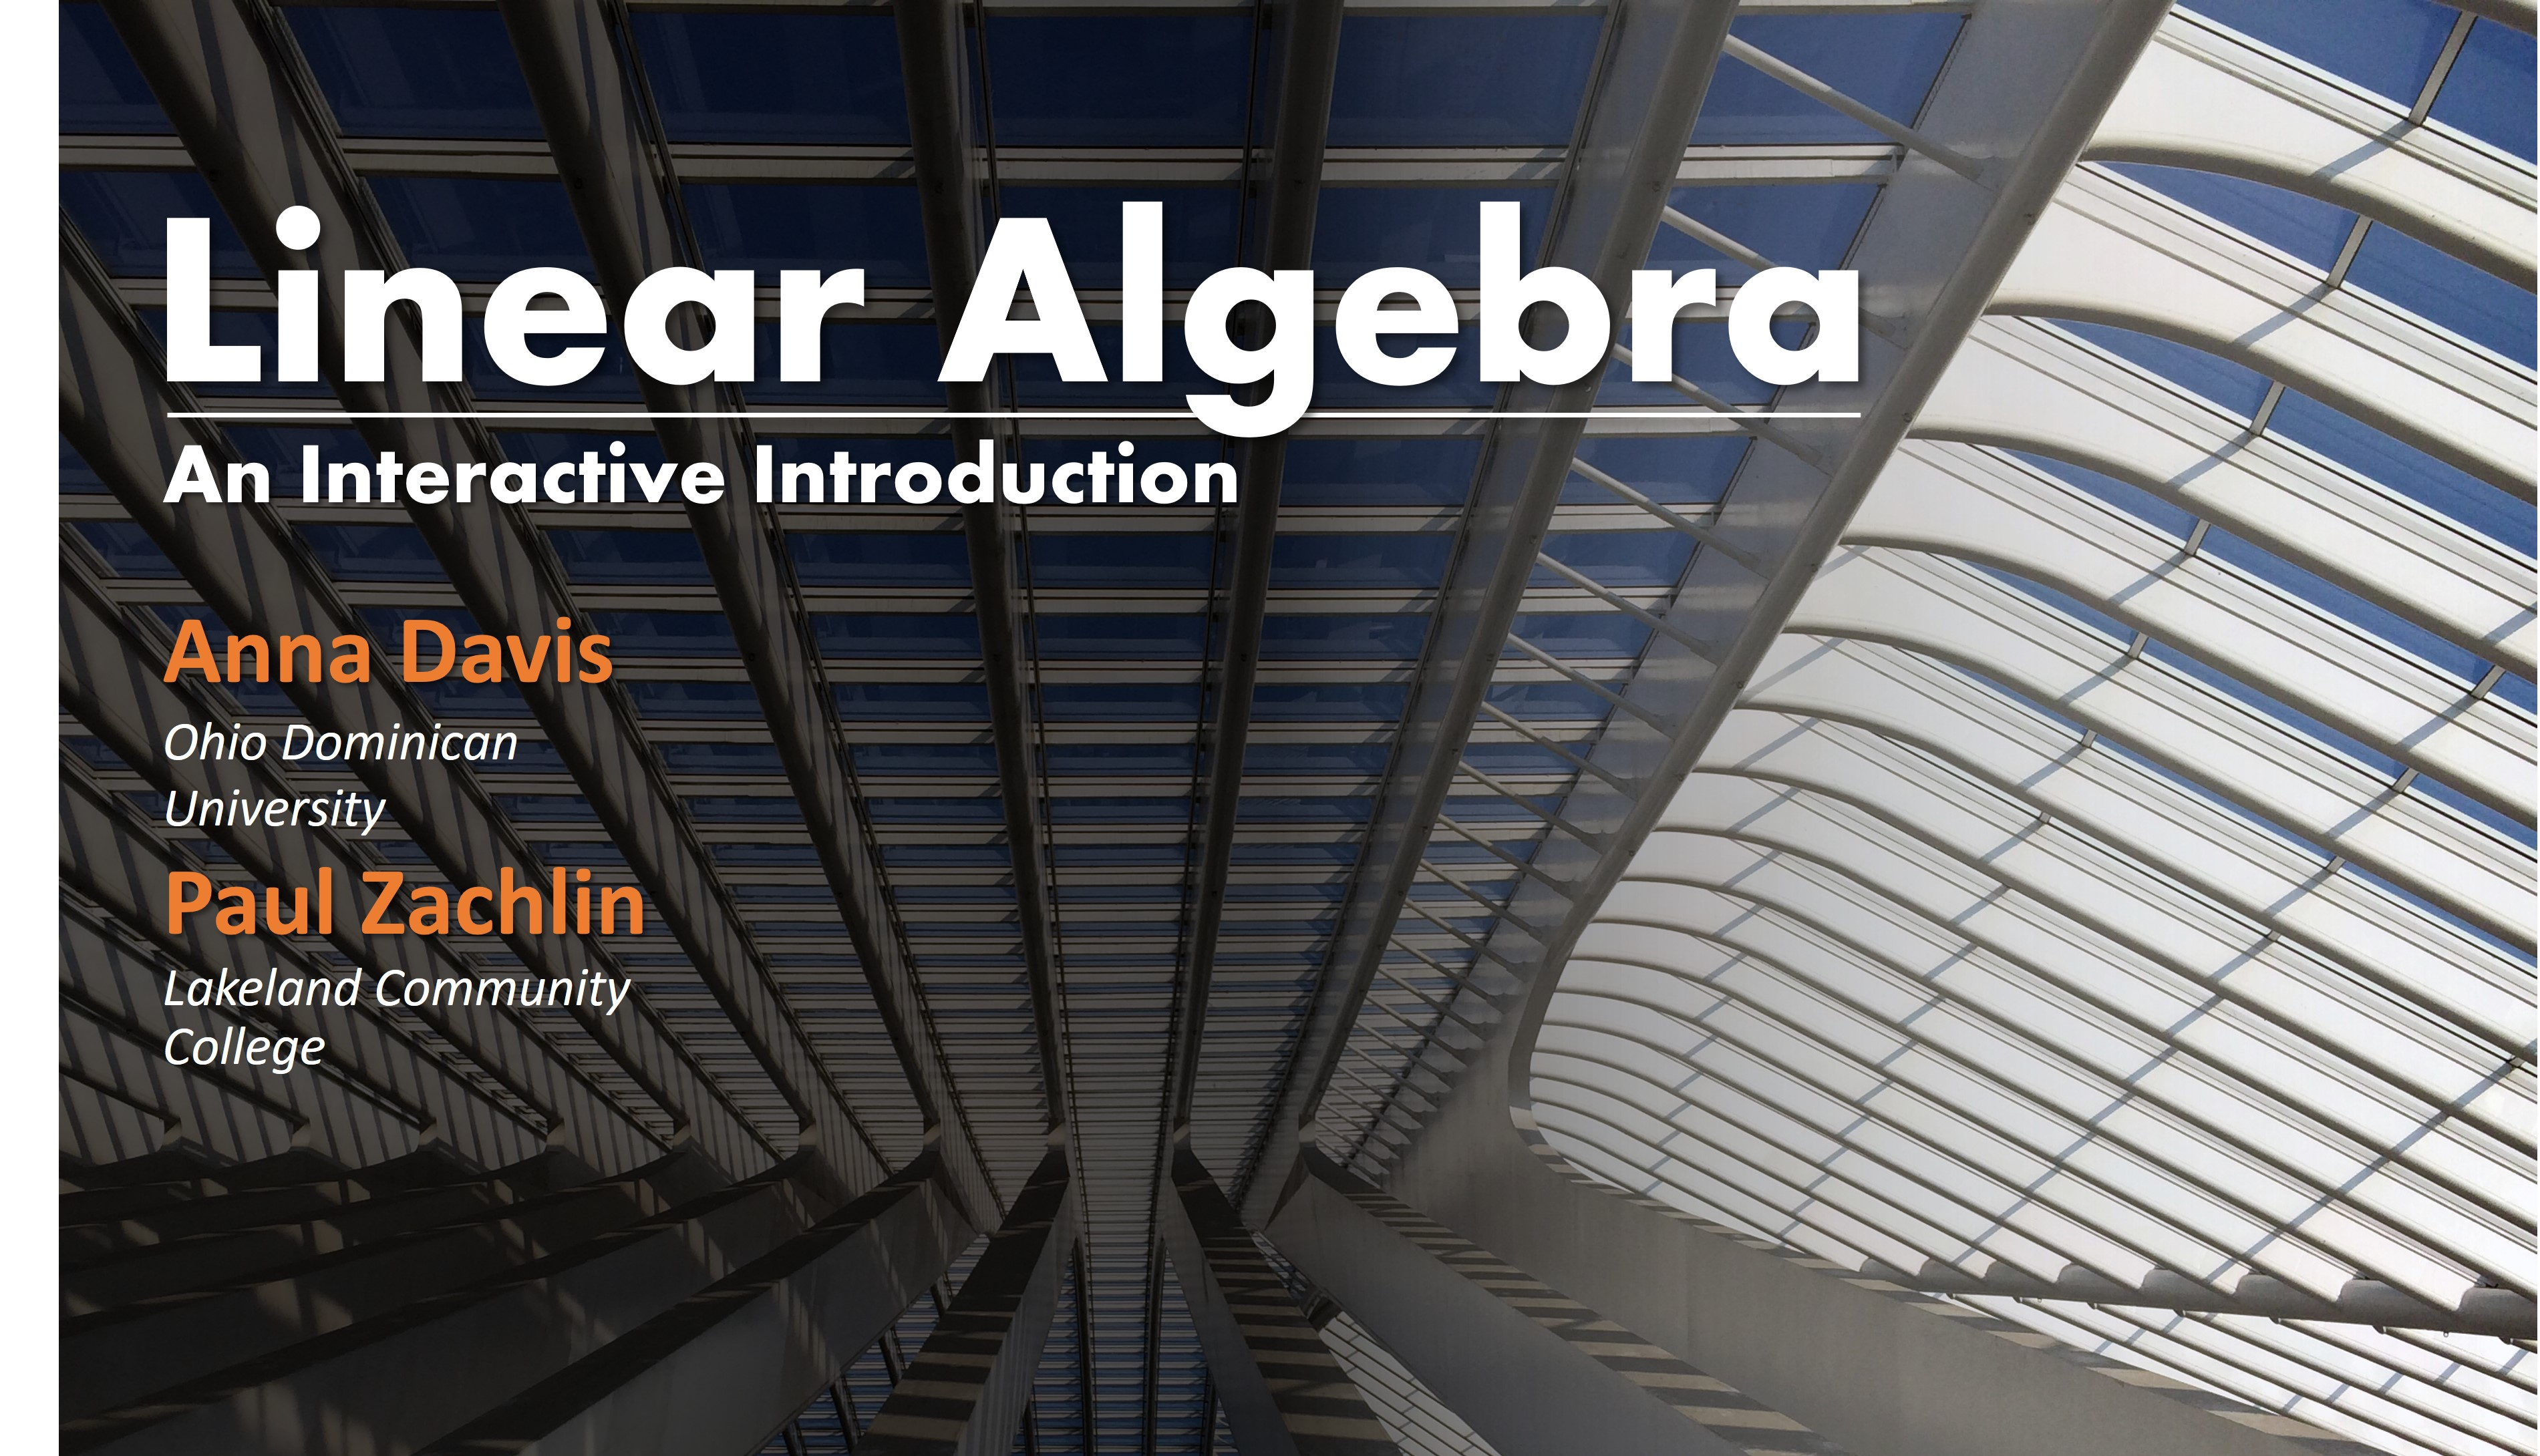
\includegraphics{BookCover1.jpg}
\end{image}

\subsection{About this Text}
This is the third edition of \emph{Linear Algebra, An Interactive Introduction}.  The \href{https://ximera.osu.edu/la/LinearAlgebra}{first edition} (2018) was funded by the Ohio Open Ed Collaborative (OOEC) through the Ohio Department of Higher Education Innovation grant. The \href{https://ximera.osu.edu/oerlinalg}{second edition} (2023) was made possible by Fall 2022 sabbatical leaves granted to Anna Davis and Paul Zachlin by Ohio Dominican University, and Lakeland Community College, respectively.

This edition contains significant updates to content, as well as formative assessments.  We have added different types of chapter review exercises, Octave exercises, and included an Octave tutorial with links to sample code.  This phase of the project was funded by the \href{https://github.com/XimeraProject}{Ximera Project} through the \href{https://www2.ed.gov/programs/otp/index.html}{Open Textbook Pilot Program} grant (2024-2026).

These materials satisfy the Ohio Transfer Module TAG Guidelines for a first course in Linear Algebra, as well as the recommendations for a first course in linear algebra made by \href{https://dx.doi.org/10.1090/noti2479}{The Linear Algebra Curriculum Study Group (LACSG 2.0)}.  

\subsection{Authors}
Anna Davis, Ohio Dominican University\\
davisa@ohiodominican.edu

Paul Zachlin, Lakeland Community College\\
pzachlin@lakelandcc.edu

With contributions from Rosemarie Emanuele of Ursuline College, and Paul Bender of Ohio Dominican University.

\subsection{Text Website}
A PDF version of this text, as well as links to previous editions of the text are available on our website \href{https://sites.google.com/view/lin-alg-interactive-intro/}{https://sites.google.com/view/lin-alg-interactive-intro/}.  The website also includes links to student and instructor surveys, as well as an errata form.

\subsection{Acknowledgements}
\begin{itemize}
\item
We would like to thank our reviewers Jim Fowler of Ohio State University and Jim Cottrill of Ohio Dominican University for their thoughtful comments and suggestions regarding the first edition.  
\item This project would not have been possible without the XIMERA platform.  Many thanks go to Bart Snapp and Jim Fowler of Ohio State University for their continued guidance and support.   
\item We would also like to thank Wim Obbels of KU Leuven, Belgium, for sharing his expertise in formatting and deploying Ximera documents.
\item We are grateful to the Ohio Open Ed Collaborative and the Ohio Department of Higher Education for providing initial funding for this project, and to Ohio Dominican University and Lakeland Community College for supporting us through sabbatical leaves, as well as the US Department of Education for funding the Ximera Project.
\item We are also grateful to Steven Valvoda for his careful reading and editing.
\item Our inspiration and some of our content came from other open textbooks. We would like to thank Keith Nicholson and Ken Kuttler for making their texts available under a Creative Commons license.  Since one of the authors taught Linear Algebra using the excellent book by David Poole for fifteen years, that text has most certainly influenced our work as well.
\end{itemize}

\section*{Bibliography}

Ken Kuttler, \href{https://open.umn.edu/opentextbooks/textbooks/a-first-course-in-linear-algebra-2017}{\it A First Course in Linear Algebra}, Lyryx 2017, Open Edition. (CC-BY)

W. Keith Nicholson, \href{https://open.umn.edu/opentextbooks/textbooks/linear-algebra-with-applications}{\it Linear Algebra with Applications}, Lyryx 2018, Open Edition. (CC-BY-NC-SA)

David Poole, {\it Linear Algebra, A Modern Introduction, 4th Edition}, Cengage Learning, 2015.  


\subsection{Questions and Comments}
For questions and comments about the content, please contact the authors.

For questions about XIMERA, please write to ximera@math.osu.edu

For anonymous feedback, and to report errata, please visit our website: \href{https://sites.google.com/view/lin-alg-interactive-intro/}{https://sites.google.com/view/lin-alg-interactive-intro/}.

\subsection{License}
This work is published under a \href{https://creativecommons.org/licenses/by-sa/4.0/deed.en}{CC-BY-SA 4.0} license.

Cover photo:  \dfn{Calatrava's beautiful structure at Guillemins railway station, Liege, Belgium} by By Elena Tatiana Chis - Own work, \href{https://creativecommons.org/licenses/by-sa/4.0/deed.en}{CC-BY-SA 4.0}.  

\href{https://commons.wikimedia.org/w/index.php?curid=60548229}{https://commons.wikimedia.org/w/index.php?curid=60548229}

\end{document}
